\section{Diagrama de Entidad Relación}

\begin{figure}
  \begin{center}
    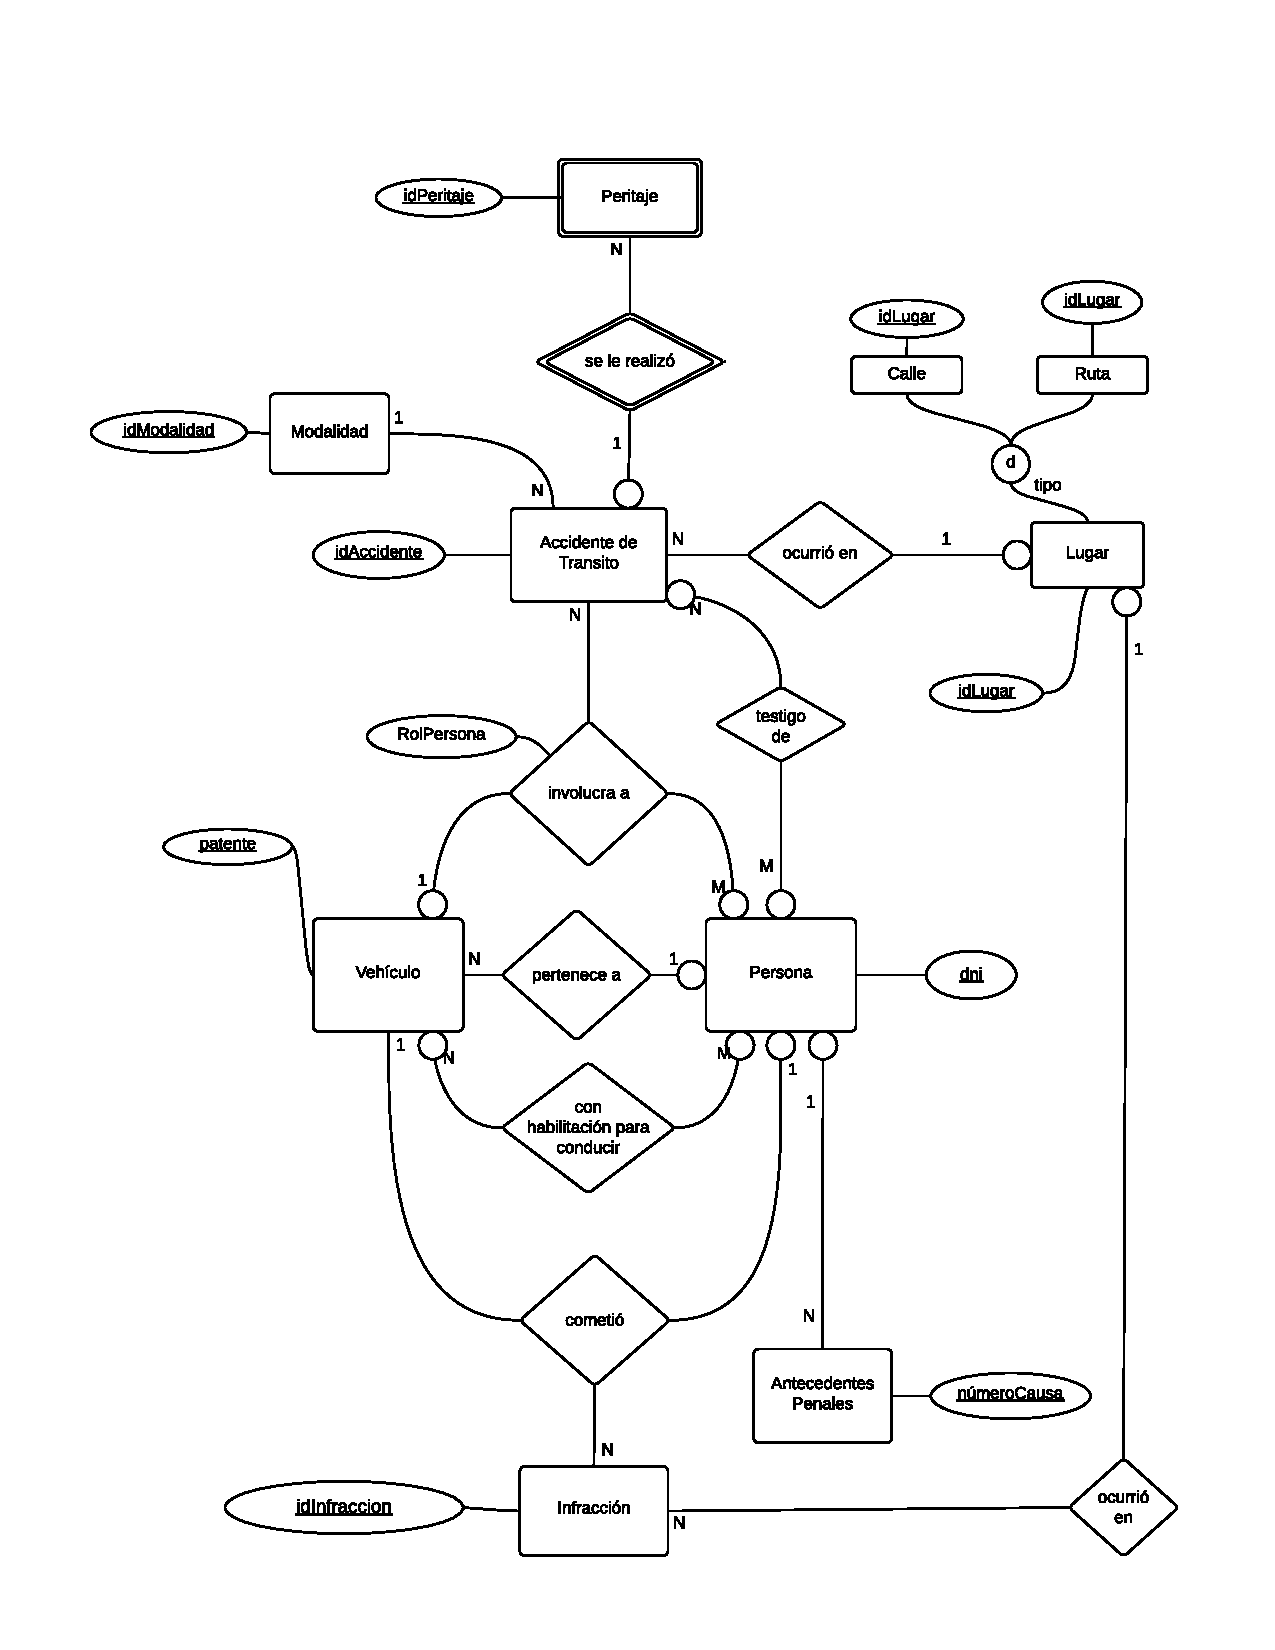
\includegraphics[scale=0.70]{diagramas/1.pdf}
    \caption{DER con PK's únicamente}
  \end{center}
\end{figure}

\subsection{Asunciones del dominio}

\begin{itemize}
  \item \textbf{DNI:} Todas las personas tienen DNI, y este es único para cada persona.
  \item \textbf{Lugar:} Los accidentes solo ocurren en calles y rutas. Por lo tanto se dividen en estas categorías(disjuntas).
  \item \textbf{Lugar:}  El tipo de pavimento de un lugar(calle o ruta) es uniforme a lo largo de toda su extensión.
  \item \textbf{Lugar:}  El tipo de pavimento de un lugar(calle o ruta) es uniforme a lo largo de toda su extensión. Es decir, no hay calles que estén asfaltadas en algunos tramos y no lo estén en otros.
  \item \textbf{Lugar:}  La velocidad máxima permitida de un lugar(calle o ruta) es uniforme a lo largo de toda su extensión.
  \item \textbf{Denuncias:}  Las denuncias policiales son tomadas por un único oficial.
  \item \textbf{Peritaje:}  Cada peritaje es realizado por un único perito.
  \item \textbf{Peritaje:}   Un peritaje consiste de un análisis de un factor relevante en el accidente. Por ejemplo, estado de iluminación de la vía al momento del accidente.
  \item \textbf{Peritaje:}  Cada peritaje tiene su resultado.
  \item \textbf{Accidente:}  Las personas tienen un único rol en un accidente: Pueden ser conductores o acompañantes de un vehículo, terceros afectados por este último o testigos. Los testigos no se relacionan con un vehículo en particular.
\end{itemize}

\subsection{DER con Primary Keys únicamente}
Como el diagrama está compuesto por muchas entidades con muchas relaciones, incluímos como primera aproximación un esqueleto
del modelo, en donde incluímos únicamente las entidades con sus claves primarias, la cardinalidad de las relaciones y
los atributos más relevantes.

\subsection{DER completo}
El diagrama completo fue separado en varias partes para facilitar su lectura.

\begin{figure}
  \begin{center}
    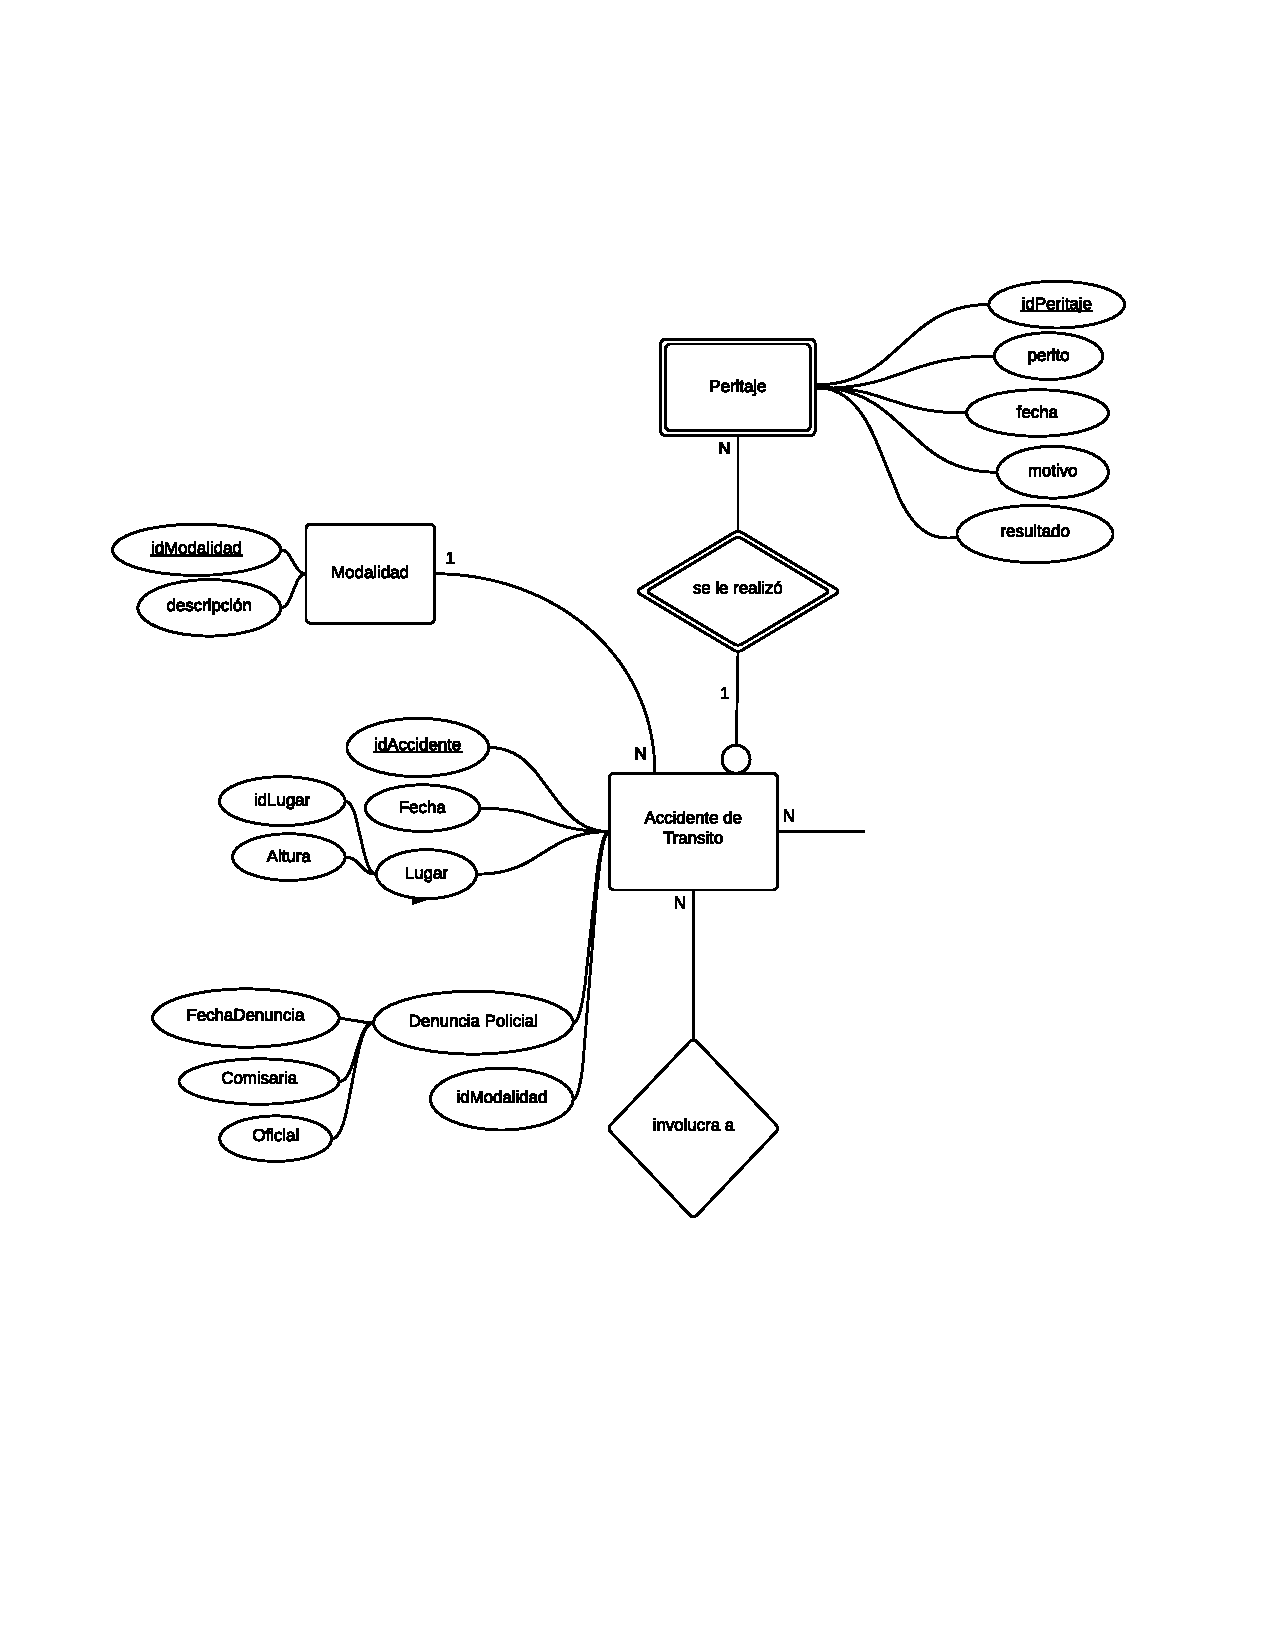
\includegraphics[scale=0.80]{diagramas/2-1.pdf}
    \caption{Accidente.Modalidad.Peritaje}
  \end{center}
\end{figure}

\begin{figure}
  \begin{center}
    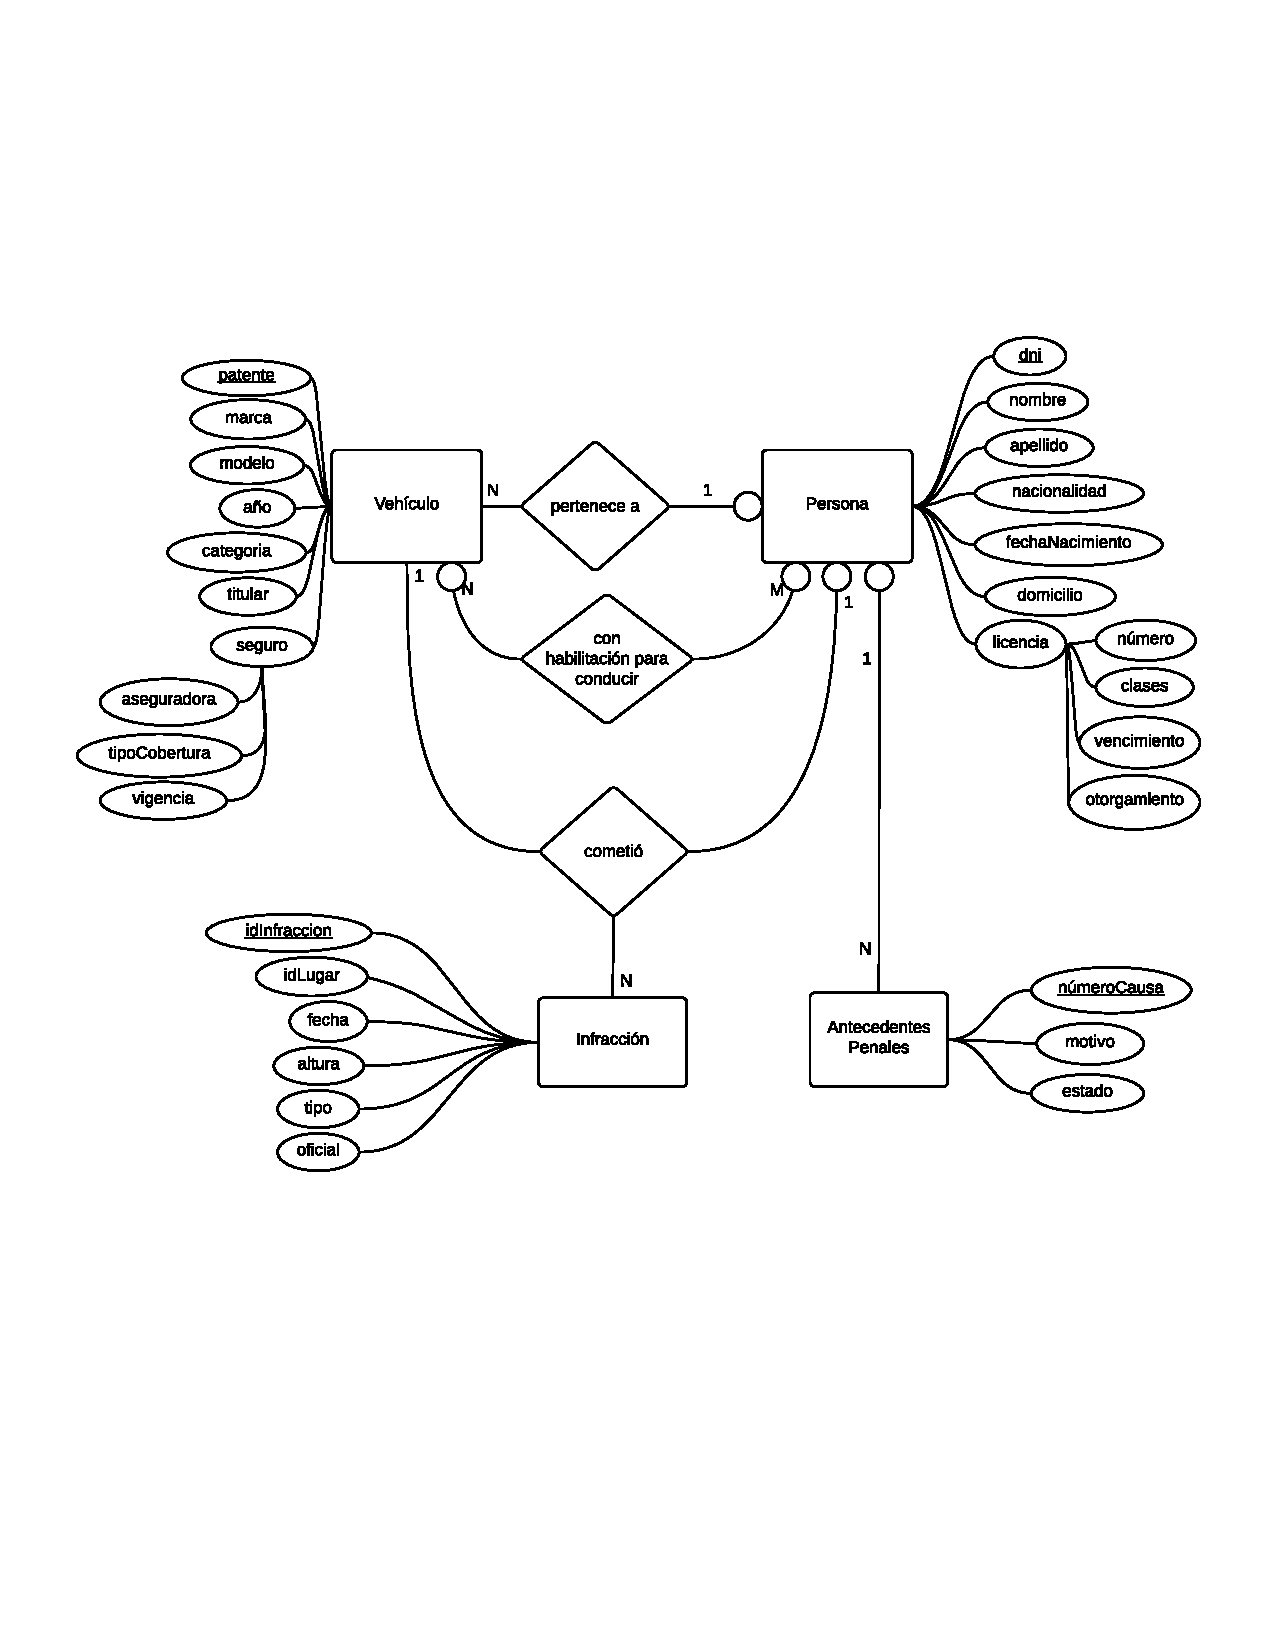
\includegraphics[scale=0.8]{diagramas/2-2.pdf}
    \caption{Vehículo.Persona.Antecedentes penales.Infracción}
  \end{center}
\end{figure}

\begin{figure}
  \begin{center}
    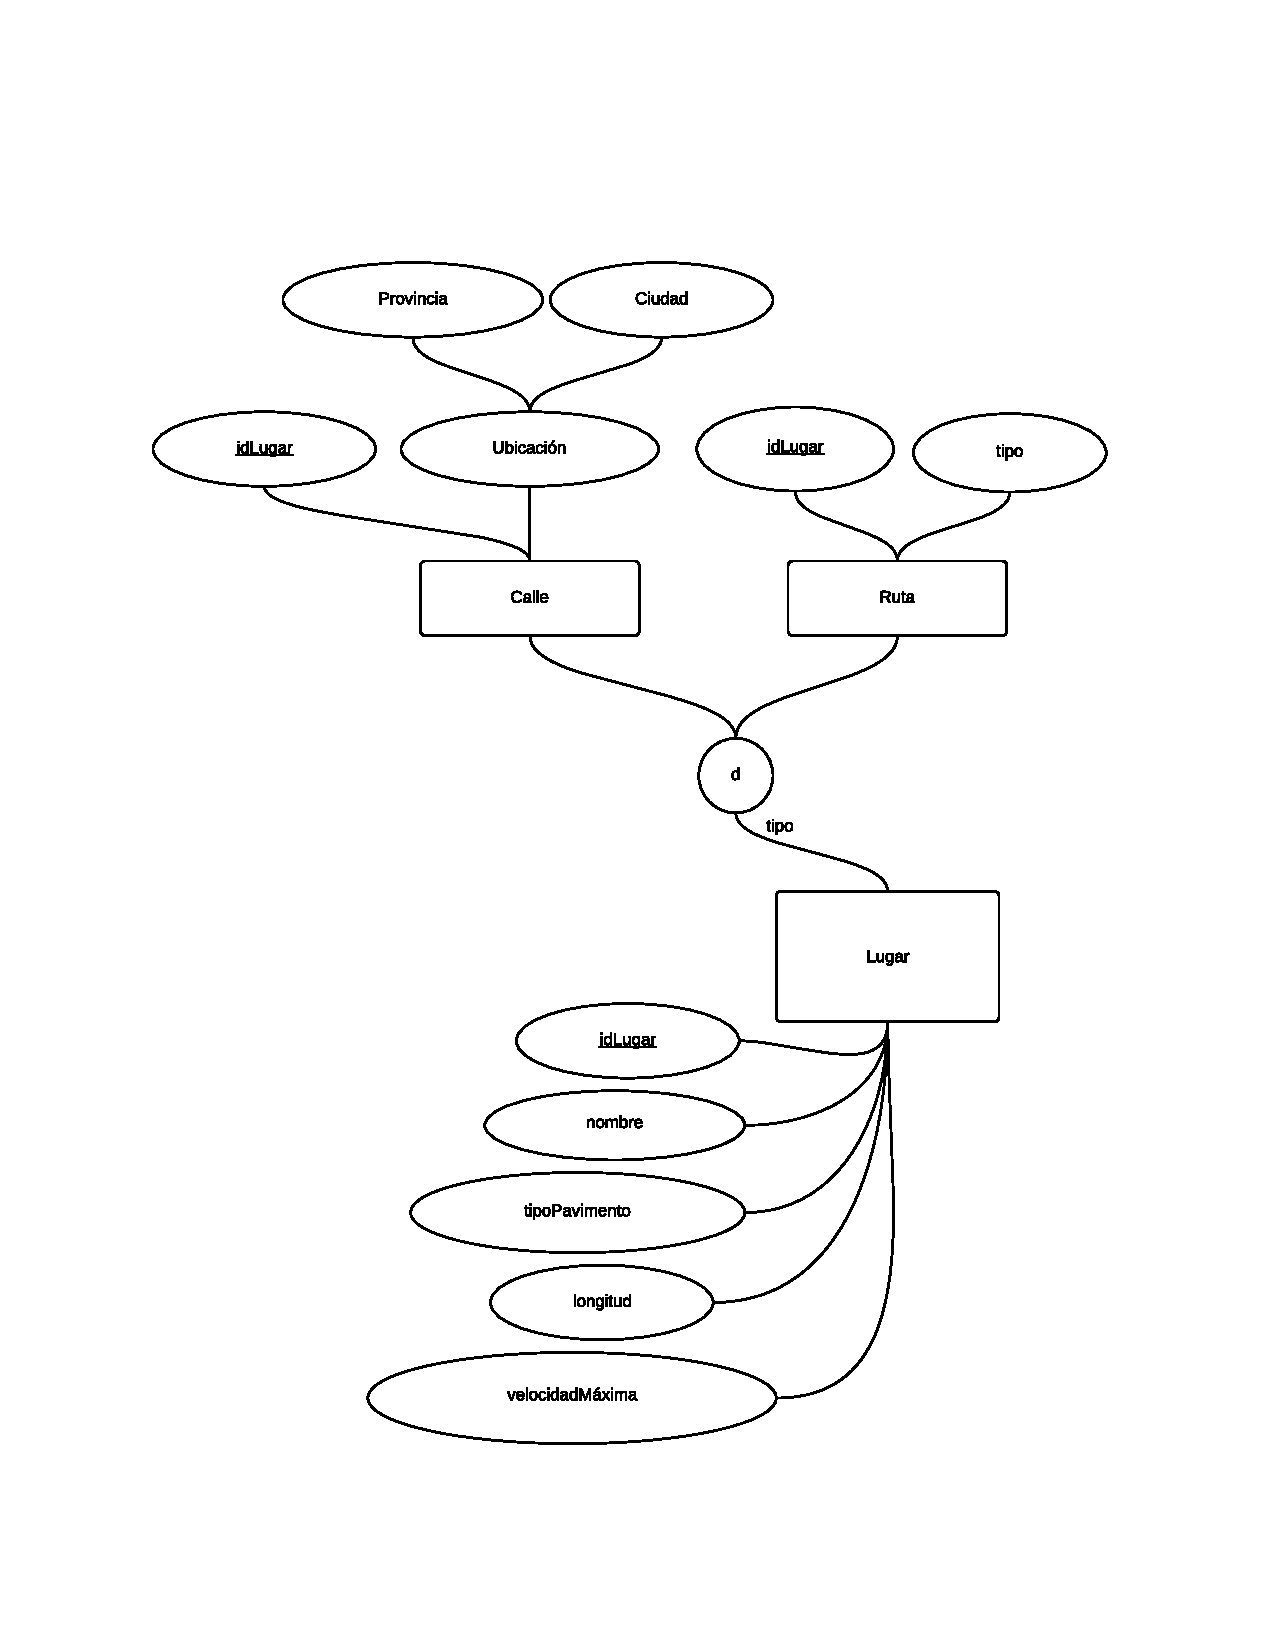
\includegraphics[scale=0.6]{diagramas/2-3.pdf}
    \caption{Lugar:Calle/Ruta}
  \end{center}
\end{figure}






